\documentclass[18pt]{beamer}
\usepackage[utf8]{inputenc} % for the umlauts
\usepackage{subfigure}

\beamertemplatenavigationsymbolsempty
%% SLIDE FORMAT

% use 'beamerthemekit' for standard 4:3 ratio
% for widescreen slides (16:9), use 'beamerthemekitwide'

\usepackage{templates/beamerthemekit}
% \usepackage{templates/beamerthemekitwide}

\setcounter{tocdepth}{1}

%% TITLE PICTURE

% if a custom picture is to be used on the title page, copy it into the 'logos'
% directory, in the line below, replace 'mypicture' with the 
% filename (without extension) and uncomment the following line
% (picture proportions: 63 : 20 for standard, 169 : 40 for wide
% *.eps format if you use latex+dvips+ps2pdf, 
% *.jpg/*.png/*.pdf if you use pdflatex)

%\titleimage{mypicture}

%% TikZ INTEGRATION

% use these packages for PCM symbols and UML classes
% \usepackage{templates/tikzkit}
% \usepackage{templates/tikzuml}

% the presentation starts here

\usepackage{mathabx}
\usepackage{picture}
\usepackage[absolute,overlay]{textpos}
%\usepackage[texcoord,grid,gridunit=mm,gridcolor=red, subgridcolor=green]{eso-pic}
\setbeamercovered{invisible}
\setbeamertemplate{caption}{\raggedright\insertcaption\par}

\title[SWT1]{Softwaretechnik 1 - 5. Tutorium}
\subtitle{Tutorium 03}
\author{Felix Bachmann}
\date{10.07.2017}

\institute{KIT - Institut für Programmstrukturen und Datenorganisation (IPD)}

% Bibliography

\usepackage[citestyle=authoryear,bibstyle=numeric,hyperref,backend=biber]{biblatex}
\addbibresource{templates/example.bib}
\bibhang1em

\begin{document}
	
% change the following line to "ngerman" for German style date and logos
\selectlanguage{ngerman}
	
%title page
\begin{frame}
\titlepage
\end{frame}

\begin{frame}
\tableofcontents
\end{frame}


\section{Orga}

	\subsection{Allgemein}
	\begin{frame}
		\frametitle{Allgemeines}
		\begin{alertblock}{Nächstes Mal letztes Tutorium} 
		\begin{itemize}
			\item irgendwelche Wünsche für das letzte Tut?
			\begin{itemize}
				\item etwas bestimmtes wiederholen?
				\item falls euch noch was einfällt, schreibt mir eine Mail
				\linebreak $\implies$ felix.bachmann@ewetel.net
			\end{itemize}
		\end{itemize}
		\end{alertblock}
		\pause
		\begin{block}{Evaluation vom letzten Mal}
			\begin{itemize}
				\item nochmal Danke fürs Mitmachen! \pause
				\item positiv: Folien, Beispiele \pause
				\item häufigster Kritikpunkt: nicht so gut lesbarer Tafelanschrieb
				\linebreak $\implies$ versuche ich besser zu machen :)
			\end{itemize}
		\end{block}
	\end{frame}

	\subsection{Feedback 4. Übungsblatt}
	\begin{frame}
		\frametitle{4. Übungsblatt Statistik}
		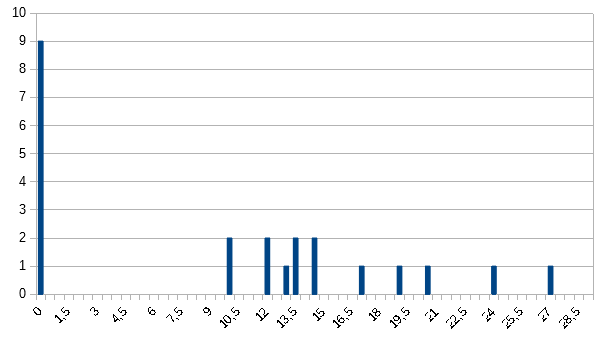
\includegraphics[scale=0.7]{./pics/tut5/statistics-ub5.png}
		\linebreak \centering $\diameter$ 13 bzw 18,4 von 25+8
	\end{frame}

	\begin{frame}
		\frametitle{4. Übungsblatt - Häufige Fehler (A3)}
		\begin{block}{Aufgabe 3 (GUI für Geometrify): 6,56 bzw. 11,25 von 10+7} 
			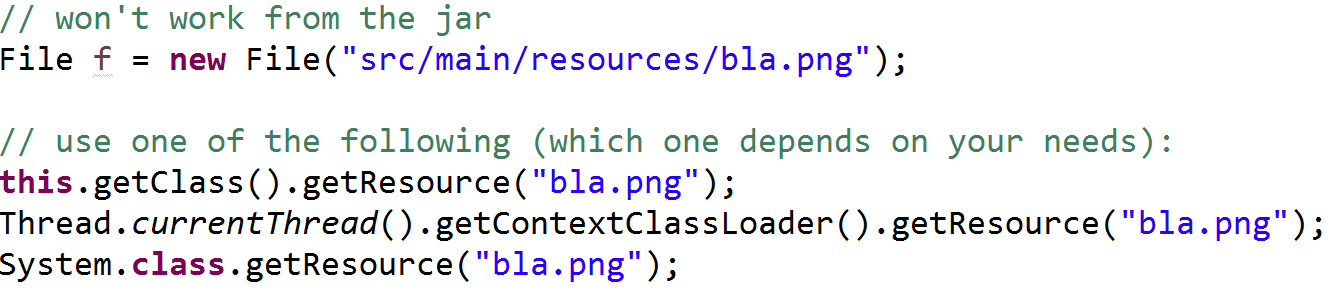
\includegraphics[scale=0.34]{./pics/tut5/file-resource.png}
			\begin{itemize}
				\pause
				\item keine leeren JPanels o.a. Objekte benutzen, um Platz zwischen Objekten zu erzeugen
				\linebreak $\implies$ geht schöner, performanter mit LayoutManagern \pause
				\item fileChooser.setFileFilter(filter) anstatt fileChooser.addChoosableFileFilter(filter)
			\end{itemize}
			\pause 
			mehr zur Aufgabe 3 nach dem Parallelität-Teil!
		\end{block}
	\end{frame}


	\subsection{Feedback 5. Übungsblatt}
	\begin{frame}
		\frametitle{5. Übungsblatt Statistik}
		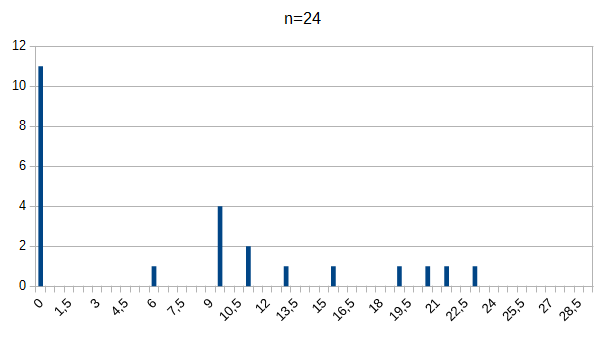
\includegraphics[scale=0.7]{./pics/tut5/statistics-ub5-2.png}
		\linebreak \centering $\diameter$ 7 bzw. 14 von 27+2
	\end{frame}

	\subsection{5. Übungsblatt - Fehler (Allgemein)}
	\begin{frame}
		\frametitle{Häufige Fehler}
		\begin{block}{Allgemein}
			\begin{itemize}
				\item (mal wieder\dots) CheckStyle und JavaDoc
			\end{itemize}
		\end{block}
	\end{frame}

	\subsection{5. Übungsblatt - Fehler}
	\begin{frame}
		\frametitle{Häufige Fehler}
		\begin{block}{Aufgabe 1 (Architekturstile): $\diameter$ 1,4 bzw. 2,79 von 4}
			\begin{itemize}
				\pause 
				\item "'Wenn wir unsere Functionality in der Cloud anbieten erhöhen wir die Customer-Reachability."'
				\linebreak $\implies$ nicht Client/Server, sondern Service Oriented Architecture (SOA) \pause
				\linebreak hatte keiner so, Übungsleiter haben Client/Server aber nicht zugelassen\dots
				\item oft vergessen:
				\begin{itemize}
					\item Wann findet zwischen wem Kommunikation statt? 
					\item Wo findet die Bildberechnung statt?
				\end{itemize}
			\end{itemize}
		\end{block}
	\end{frame}

	\begin{frame}
		\frametitle{Häufige Fehler}
		\begin{block}{Aufgabe 2 (Iterator für Plug-Ins): $\diameter$ 1,4 bzw. 4,19 von 6}
			\begin{itemize}
				\pause 
				\item Klasse PluginManager als "'Klient/Kontext"' im UML-Diagramm vergessen \pause
				\item Sortierung der Liste sollte \textbf{im} Iterator \textbf{sichergestellt} werden
			\end{itemize}
		\end{block}
		\pause 
		\begin{block}{Aufgabe 3 (Umstrukturierung von Geometrify): $\diameter$ 2,69 bzw. 5,38 von 8}
			\begin{itemize}
				\item (abstrakte) Fabrik $\ne$ Fabrikmethode \pause
				\item  kein Beobachter, sondern Memento \pause
				\item Entwurfsmuster-Elemente im UML-Diagramm nicht richtig markiert \pause
				\item richtige Muster verwendet, falsche Muster erklärt \pause
				\item getPrimitive() ist Einschubmethode im Schablonenmethoden-Muster \textbf{UND} Fabrikmethode im Fabrikmethoden-Muster
			\end{itemize}
		\end{block}
	\end{frame}

	\begin{frame}
		\frametitle{Häufige Fehler}
		\begin{block}{Aufgabe 4 (Reimplementierung von Geometrify): $\diameter$ 1,92 bzw. 6,57 von 7+2}
			\begin{itemize}
				\pause
				\item Bonus (nicht achsensymmetrische Rechtecke) nicht gemacht
			\end{itemize}
		\end{block}
		\pause
		\begin{block}{Aufgabe 5 (GUI-Erweiterung): $\diameter$ 0,04 bzw. 1 von 2}
			\begin{itemize}
				\item \textbf{EINE} Abgabe :D
			\end{itemize}
		\end{block}
	\end{frame}

	\begin{frame}
		\frametitle{Jetzt letztes Übungsblatt..}
		\begin{huge}
			Falls ihr noch Punkte braucht, gebt ab!
		\end{huge}
\end{frame}

\section{Überblick}
	\subsection{Überblick}
	\begin{frame}
		\frametitle{Überblick}
		\begin{huge}
			Wo sind wir?
		\end{huge}
	\end{frame}
	
	
	
\section{Parallelität}
	\subsection{}	
	
	\begin{frame}
		\frametitle{Parallelität - Grundlagen}
		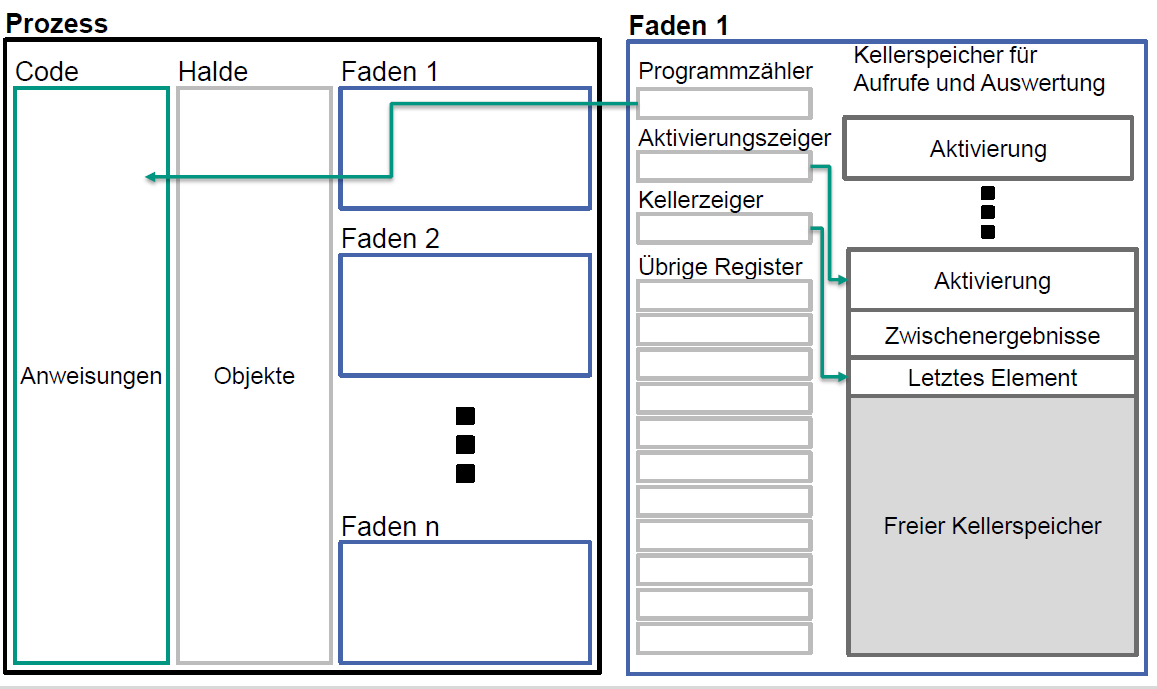
\includegraphics[scale=0.34]{./pics/tut5/proc-thr.png}
	\end{frame}

	\begin{frame}
		\frametitle{Parallelität - Grundlagen}
		\begin{itemize}
			\item Prozess = Programm in Ausführung \pause
			\item jeder Prozess hat eigenen Adressraum (= Speicherbereich im Arbeitsspeicher) \pause
			\item jeder Prozess hat mindestens einen Thread \pause
			\item Threads existieren innerhalb eines Prozesses \pause 
			\begin{itemize}
				\item Threads haben den gleichen Heap und Code \pause 
					\linebreak $\implies$ alle Threads innerhalb eines Prozesses arbeiten mit denselben Objekten und demselben Code \pause 
				\item Threads haben eigene Stacks und Befehlszeiger (Programmzähler) \pause 
					\linebreak $\implies$ Threads haben eigene lokale Variablen und können beliebigen Code des Prozesses ausführen
			\end{itemize}
		\end{itemize}
	\end{frame}
	
	
	\begin{frame}
		\frametitle{Parallelität - Motivation}
		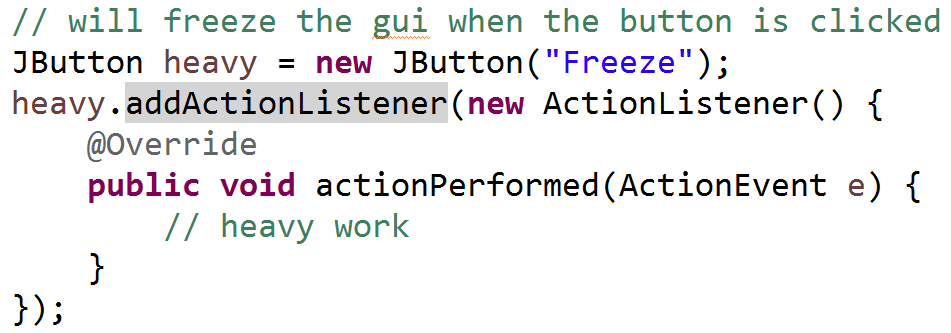
\includegraphics[scale=0.34]{./pics/tut5/mot-par.png}
		\pause
		\begin{itemize}
			\item "'normales"' sequentielles Programm = 1 Prozess mit 1 Thread
			\item paralleles Programm = 1 Prozess mit mehreren Threads
		\end{itemize}
	\end{frame}

	\begin{frame}
		\frametitle{Parallelität - in Java}
		\begin{itemize}
			\item in Java zwei Möglichkeiten einen Thread zu erstellen
			\item bereits in Java enthalten:
			\begin{itemize}
				\item Interface java.lang.Runnable
				\item Klasse java.lang.Thread
			\end{itemize}
		\end{itemize}
	\end{frame}

	\begin{frame}
		\frametitle{Parallelität - in Java}
		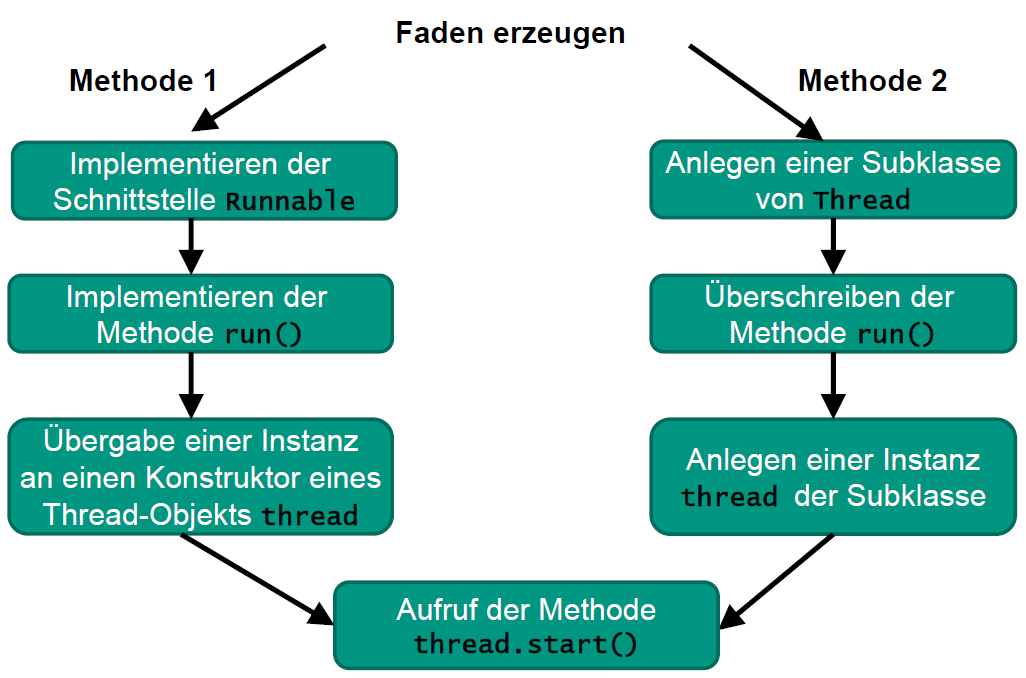
\includegraphics[scale=0.34]{./pics/tut5/crea-thr.png}
	\end{frame}

	\begin{frame}
		\frametitle{Parallelität - in Java}
		\centering
		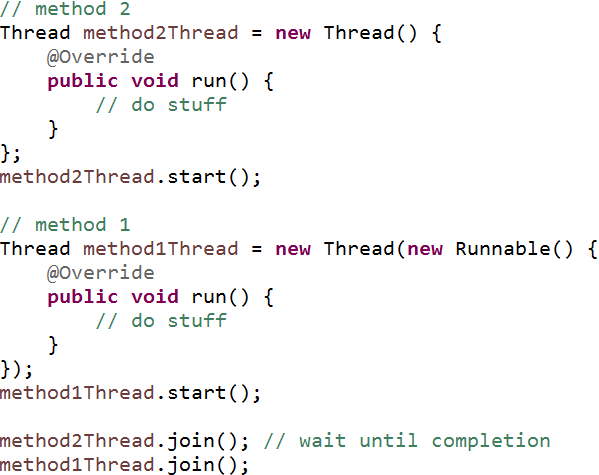
\includegraphics[scale=0.43]{./pics/tut5/crea-thr-java.png}
		\pause
		\begin{alertblock}{Wichtig!}
			\begin{itemize}
				\item immer Thread.start() aufrufen, nicht Thread.run() \pause
				\item Thread.run() würde run() sequenziell aufrufen, start() kehrt direkt zurück, nachdem Thread gestartet wurde
			\end{itemize}
		\end{alertblock}
	\end{frame}

	\begin{frame}
		\frametitle{Parallelität - Synchronisation}
		\begin{itemize}
			\item Problem: Zugriff auf globale Variablen/ Objekte passiert nicht parallel, Unterbrechungen möglich
			\item Folge: ggf. falsche Ergebnisse
		\end{itemize}
		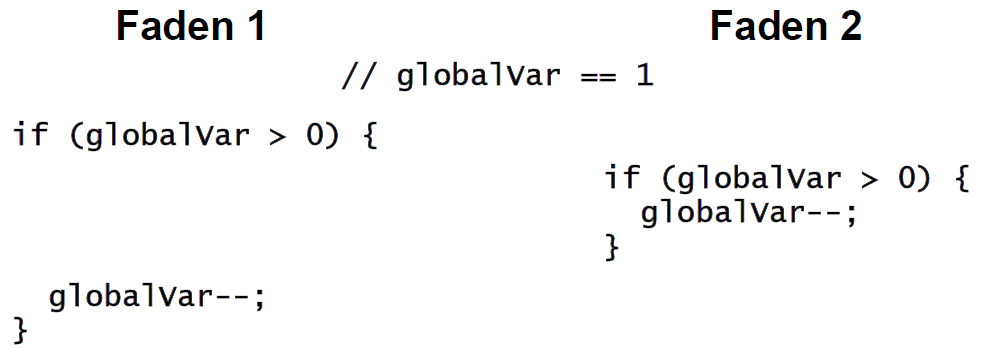
\includegraphics[scale=0.43]{./pics/tut5/par-pro.png}
	\end{frame}

	\begin{frame}
		\frametitle{Parallelität - Synchronisation}
		\begin{itemize}
			\item nicht nur ein theoretisches Beispiel!
		\end{itemize}
		\centering
		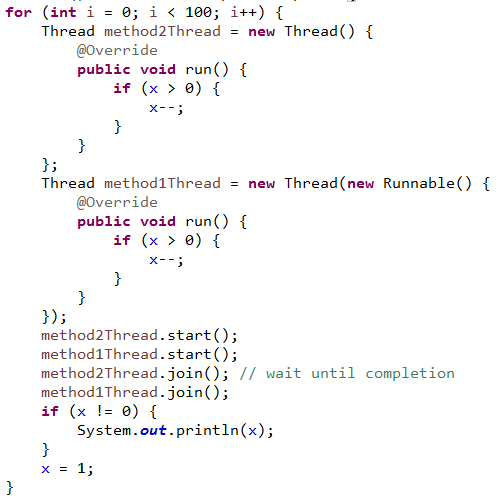
\includegraphics[scale=0.43]{./pics/tut5/synch-ex.png} \pause
		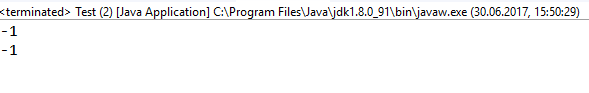
\includegraphics[scale=0.43]{./pics/tut5/synch-ex2.png}
	\end{frame}

	\begin{frame}
		\frametitle{Parallelität - Synchronisation}
		\begin{itemize}
			\item Ziel: Zugriff auf gemeinsam genutzte Daten synchronisieren \pause 
			\begin{itemize}
				\item kritische Abschnitte schützen \pause
				\item Wettlaufsituationen vermeiden
			\end{itemize}
			\begin{block}{Kritischer Abschnitt (critical section)}
				Codeabschnitt, wo Zugriffe auf gemeinsam genutzte Daten stattfinden
			\end{block} \pause
			\begin{block}{Wettlaufsituation (race condition)}
				Verhalten des Programms hängt von der zeitlichen Abfolge der Operationen ab (Wann wird welcher Thread abgebrochen?)
			\end{block} \pause
			\item Idee: Monitor einführen
		\end{itemize}
	\end{frame}

	\begin{frame}
		\frametitle{Parallelität - Monitor}
		\begin{itemize}
			\item Idee: Monitor einführen \pause
			\item Bereich im Code markieren, den nur ein Thread gleichzeitig ausführen kann und dabei nicht unterbrochen werden kann \pause
			\item Schlüsselwort in Java \textcolor{blue}{synchronized} \pause
			\item es wird immer an einem Objekt synchronisiert, als Argument bei \textcolor{blue}{synchronized} \pause
			\item Thread t kommt an eine mit \textcolor{blue}{synchronized}(Objekt)\{\dots\} markierte Stelle \pause
			\begin{itemize}
				\item es wird geprüft, ob der Monitor Objekt gerade frei ist \pause
				\item ist der Monitor frei, kommt t in den kritischen Abschnitt und der Monitor ist besetzt, bis t den Abschnitt wieder verlässt \pause
				\item ist der Monitor besetzt, wird t blockiert, bis der kritische Abschnitt frei ist
			\end{itemize}
		\end{itemize}
	\end{frame}

	\begin{frame}
		\frametitle{Parallelität - Monitor}
		private Object o = new Object();
		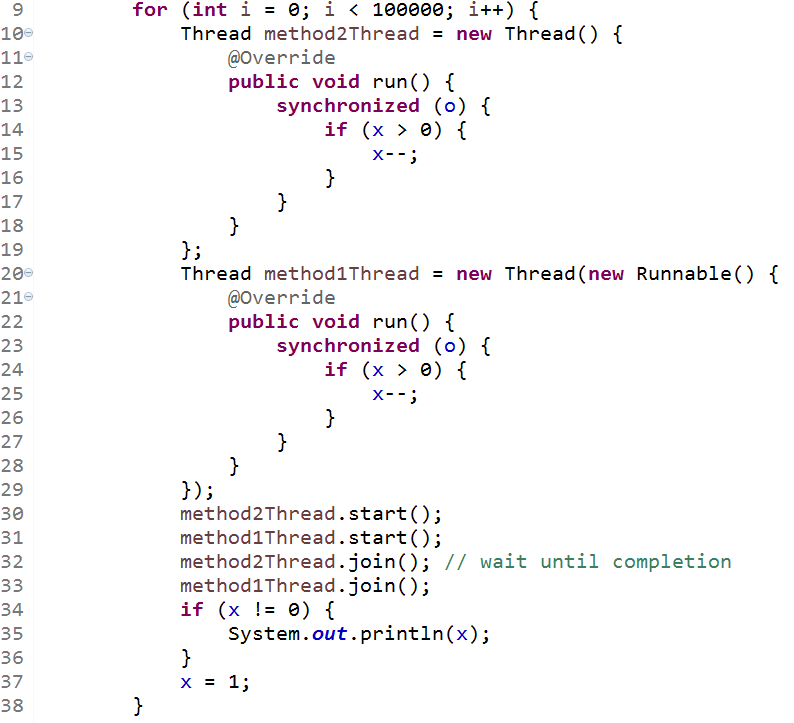
\includegraphics[scale=0.36]{./pics/tut5/synch-ex3.png} \pause
		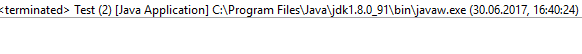
\includegraphics[scale=0.39]{./pics/tut5/synch-ex4.png}
	\end{frame}

	\begin{frame}
		\frametitle{Parallelität - wait() und notify()}
		\textcolor{blue}{synchronized} an Methoden = synchronized(this)\{Methoden-Rumpf\} \pause
		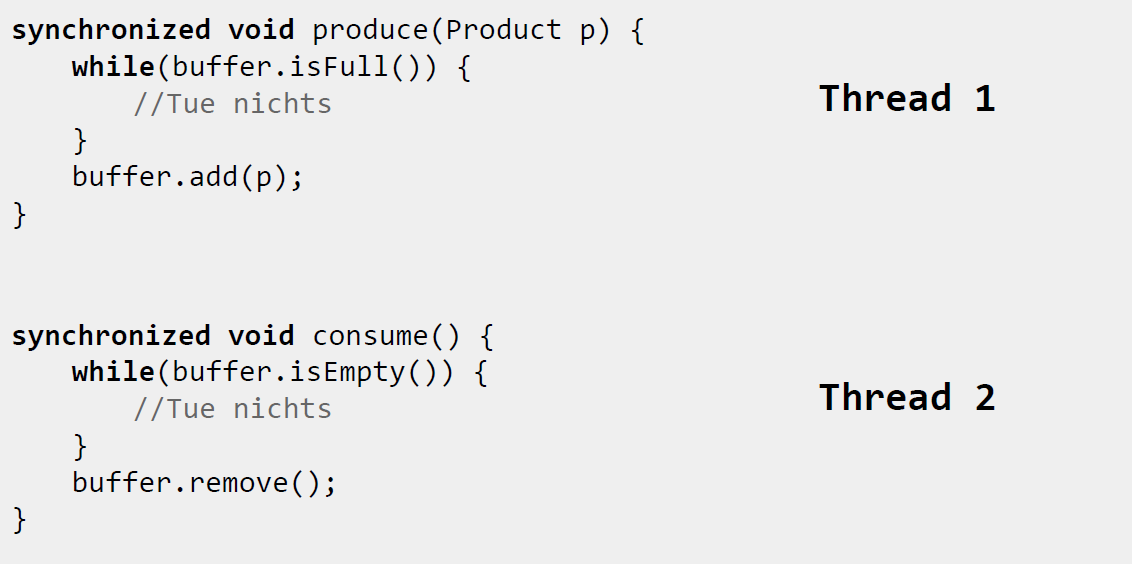
\includegraphics[scale=0.3]{./pics/tut5/cons-prod.png}
		\begin{alertblock}{Probleme}
			\begin{itemize}
				\pause
				\item "'busy waiting"' verschwendet Rechenzeit \pause
				\item wartender Produzent blockiert Konsument, der dann nichts konsumieren kann 
			\end{itemize}
		\end{alertblock}
	\end{frame}

	\begin{frame}
		\frametitle{Parallelität - wait() und notify()}
		\begin{itemize}
			\item Idee: brauchen Mechanismus, der es erlaubt den Monitor freizugeben, während man auf etwas wartet \pause
			\item dazu braucht man natürlich auch einen Mechanismus, der es erlaubt wartende Threads aufzuwecken \pause
			\item in Java: wait() und notify() bzw. notifyAll() \pause
			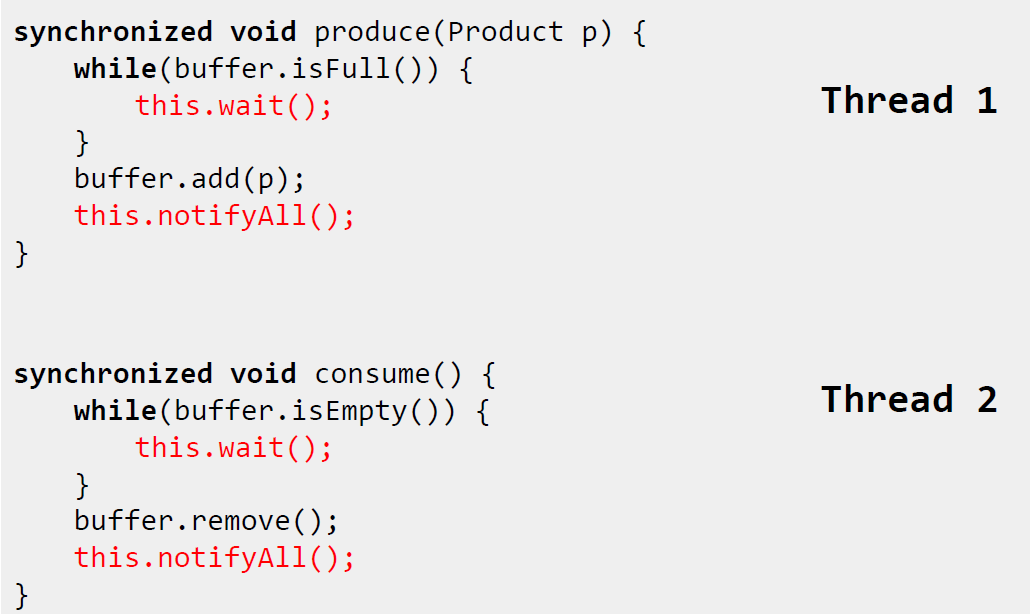
\includegraphics[scale=0.3]{./pics/tut5/cons-prod-sol.png}
		\end{itemize}
	\end{frame}

	\begin{frame}
		\frametitle{Parallelität - wait() und notify()}
		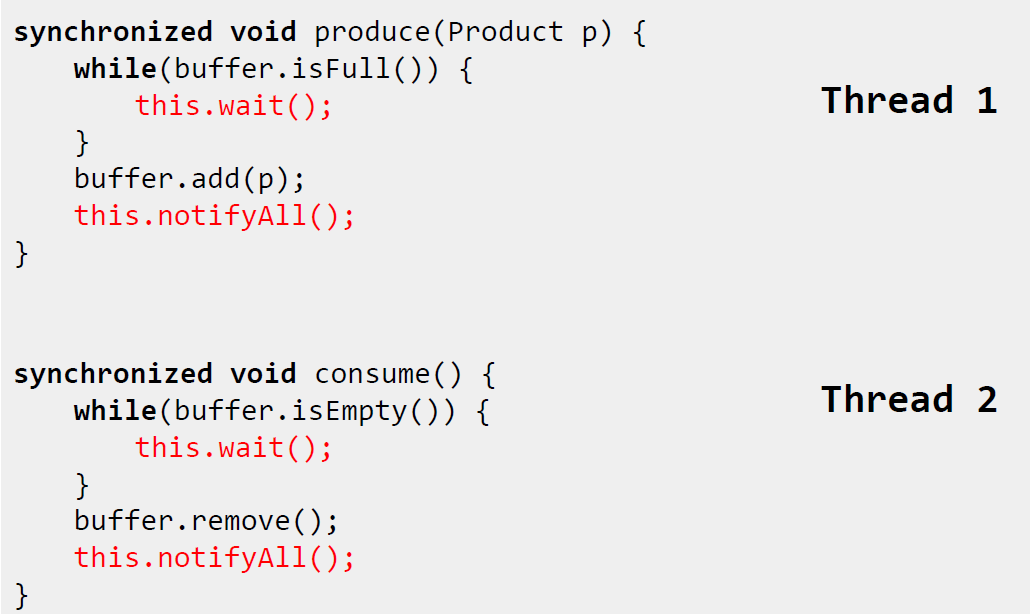
\includegraphics[scale=0.3]{./pics/tut5/cons-prod-sol.png}
		\begin{itemize}
			\item Kann man die while-Schleifen jetzt nicht durch eine if-Abfrage ersetzen? \pause
			\begin{itemize}
				\item Nein, dann würde nach dem Aufwecken nicht nochmal geprüft werden, ob die Bedingung mittlerweile falsch ist.
			\end{itemize}
		\end{itemize}
	\end{frame}

	\begin{frame}
		\frametitle{Parallelität - Verklemmung (deadlock)}
		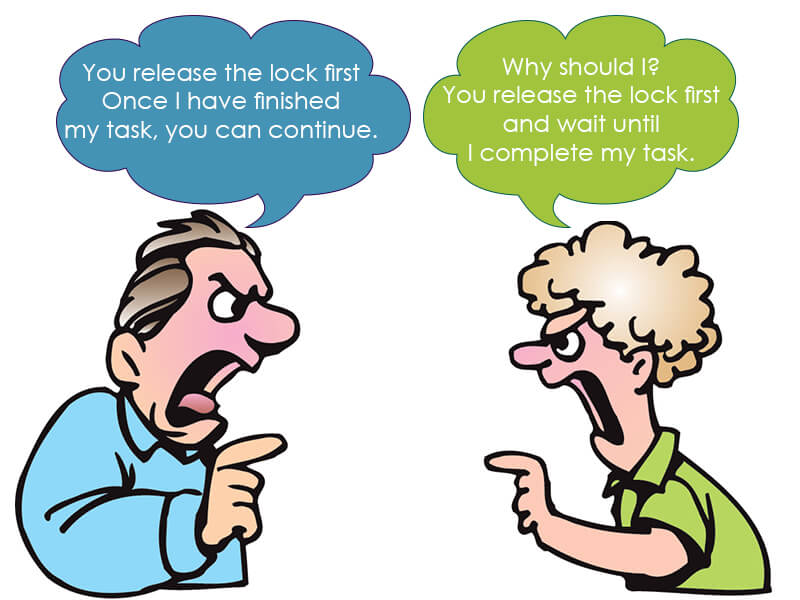
\includegraphics[scale=0.3]{./pics/tut5/deadlock.jpg}
		\pause
		\begin{itemize}
			\item Thread A hält Monitor B und benötigt Monitor C
			\item Thread B hält Monitor C und benötigt Monitor B
		\end{itemize}
	\end{frame}

	\begin{frame}
		\frametitle{Parallelität - Verklemmung (deadlock)}
			\centering 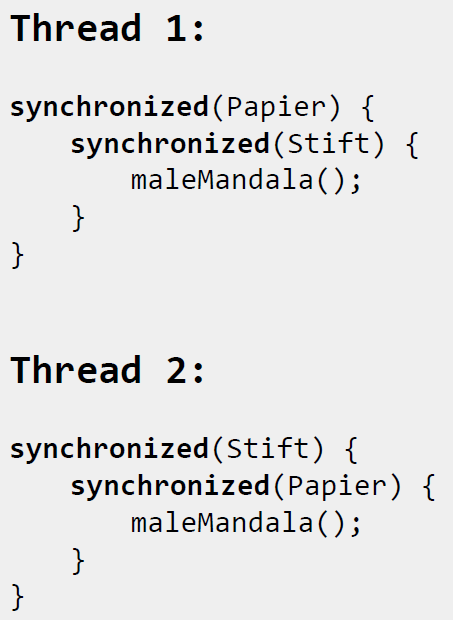
\includegraphics[scale=0.4]{./pics/tut5/deadlock-ex.png} \linebreak
			klassicher Deadlock!
	\end{frame}

	
	\begin{frame}
		\frametitle{Parallelität - Verklemmung (deadlock)}
		\centering Lösungsansatz: Monitore immer in gleicher Reihenfolge anfordern \linebreak
		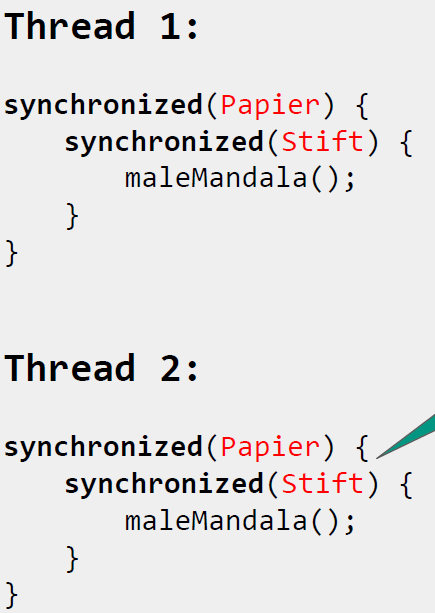
\includegraphics[scale=0.4]{./pics/tut5/deadlock-ex-sol.png}
	\end{frame}
	
	\begin{frame}
		\centering
		\begin{huge}
			Klausuraufgabe SS14
		\end{huge}
	\end{frame}
	
	
	\begin{frame}
		\frametitle{4. Übungsblatt - A3 mit Threads}
		\begin{block}{Aufgabe 3 (GUI für Geometrify): 6,56 bzw. 11,25 von 10+7} 
			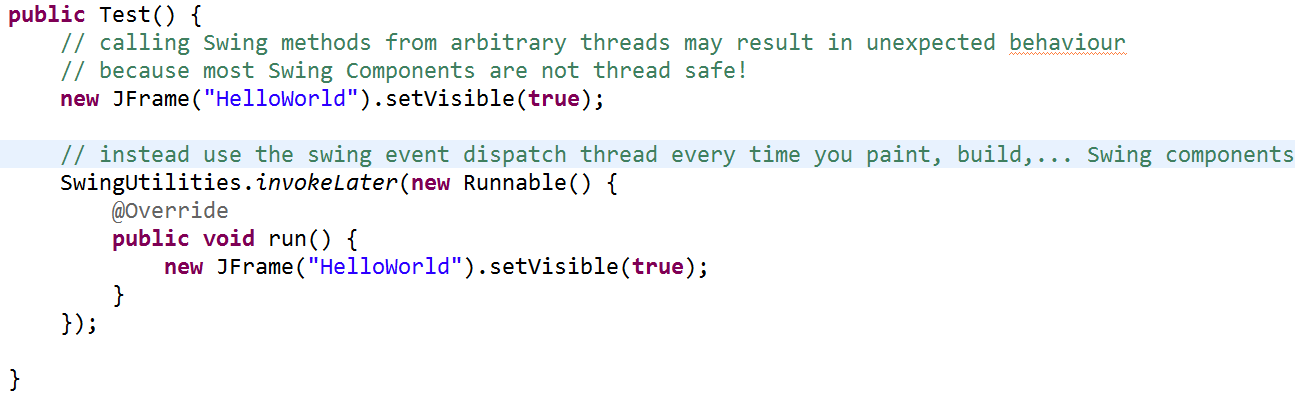
\includegraphics[scale=0.34]{./pics/tut5/edt.png}
		\end{block}
		\begin{tiny}
			siehe auch: \url{https://docs.oracle.com/javase/tutorial/uiswing/concurrency/dispatch.html}
		\end{tiny}
	\end{frame}

	\begin{frame}
		\frametitle{4. Übungsblatt - A3 mit Threads}
		\begin{block}{Aufgabe 3 (GUI für Geometrify): 6,56 bzw. 11,25 von 10+7} 
			\centering
			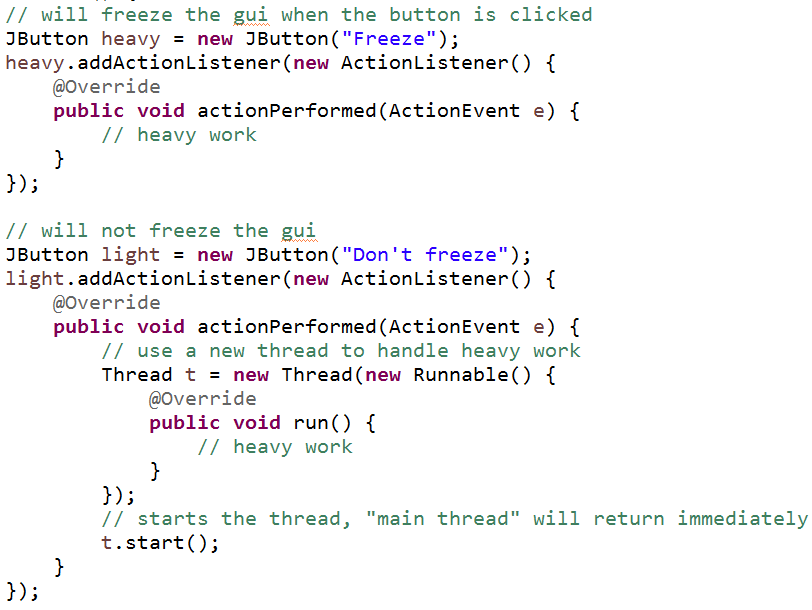
\includegraphics[scale=0.34]{./pics/tut5/extra-thread.png}
		\end{block}
	\end{frame}

\section{Testen}
	\subsection{Intro}
	
	\begin{frame}
		\frametitle{Arten von Fehlern}
		\begin{itemize}
			\item Was verursacht was?
			\item Defekt, Irrtum, Versagen \pause
			\item "'Testing shows the presence of bugs, not their absence."' (Edsger W. Dijkstra)
		\end{itemize}
	\end{frame}

	\begin{frame}
		\frametitle{Arten von Tests}
		\begin{block}{Dynamische Verfahren}
			\begin{itemize}
				\item Testfälle schreiben und ausführen (z.B. mit JUnit) \pause
				\item white box testing \pause
				\begin{itemize}
					\item kontrollflussorientiert
					\item datenflussorientiert
				\end{itemize}
				\item black box testings \pause
				\begin{itemize}
					\item funktionale Tests \pause
					\item Leistungstests
				\end{itemize}
			\end{itemize}
		\end{block}
		\pause
		\begin{block}{Statische Verfahren}
			\begin{itemize}
				\item Inspektion \pause
				\item statische Analyse mit Tools \pause
				\item Programm wird nicht ausgeführt!
			\end{itemize}
		\end{block}
	\end{frame}

	\begin{frame}
		\frametitle{Kontrollflussorientiertes Testverfahren (KFO)}
		Vorgehen:
		\begin{enumerate}
			\item gegeben: zu testender Code \pause
			\item Code $\implies$ Zwischensprache
			\begin{itemize}
				\item Sprünge umwandeln
				\item Grundblöcke finden
				\item Grundblöcke prüfen
			\end{itemize}
			\pause
			\item Zwischensprache $\implies$ Kontrollflussgraph \pause
			\item am Kontrollflussgraphen testen: \pause
			\begin{itemize}
				\item Anweisungsüberdeckung
				\item Zweigüberdeckung 
				\item Pfadüberdeckung
			\end{itemize}
		\end{enumerate}
	\end{frame}

	\begin{frame}
		\frametitle{KFO: Code nach Zwischensprache}
		\begin{itemize}
			\item Sprünge umwandeln
		\end{itemize}
		\centering 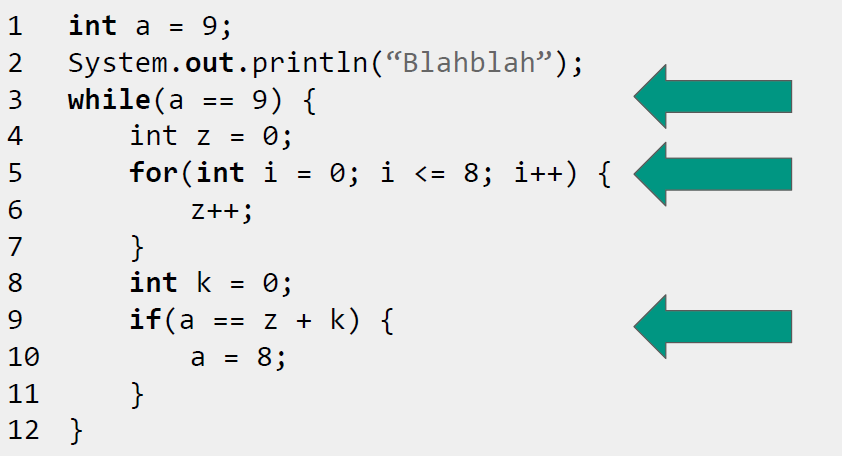
\includegraphics[scale=0.34]{./pics/tut5/code.png}
	\end{frame}

	\begin{frame}
		\frametitle{KFO: Code nach Zwischensprache}
		\begin{itemize}
			\item Sprünge umwandeln
		\end{itemize}
		\centering 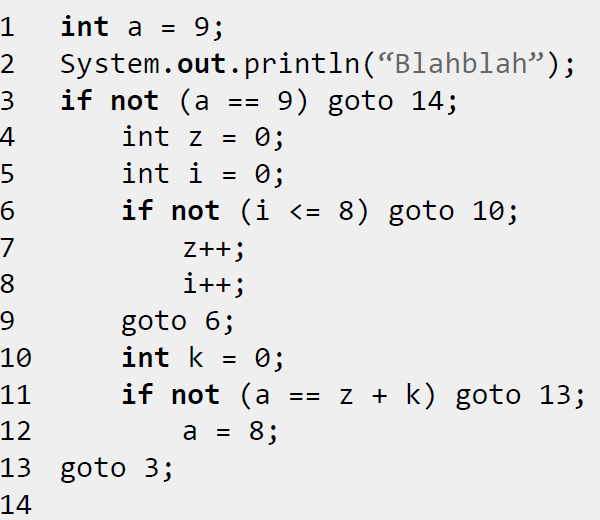
\includegraphics[scale=0.34]{./pics/tut5/code-jumps.png}
	\end{frame}

	\begin{frame}
		\frametitle{KFO: Code nach Zwischensprache}
		\begin{itemize}
			\item Grundblöcke finden (Code bis goto ist ein Grundblock)
		\end{itemize}
		\centering 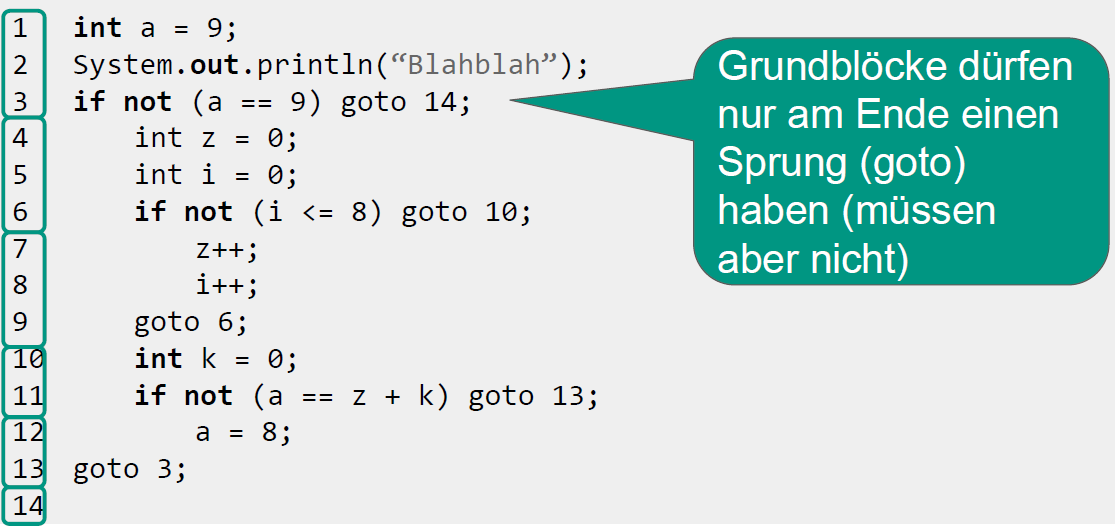
\includegraphics[scale=0.34]{./pics/tut5/first-blocks.png}
	\end{frame}

	\begin{frame}
		\frametitle{KFO: Code nach Zwischensprache}
		\begin{itemize}
			\item 	Grundblöcke prüfen (goto dürfen nur an Anfang eines Grundblocks verweisen)
		\end{itemize}
			\centering 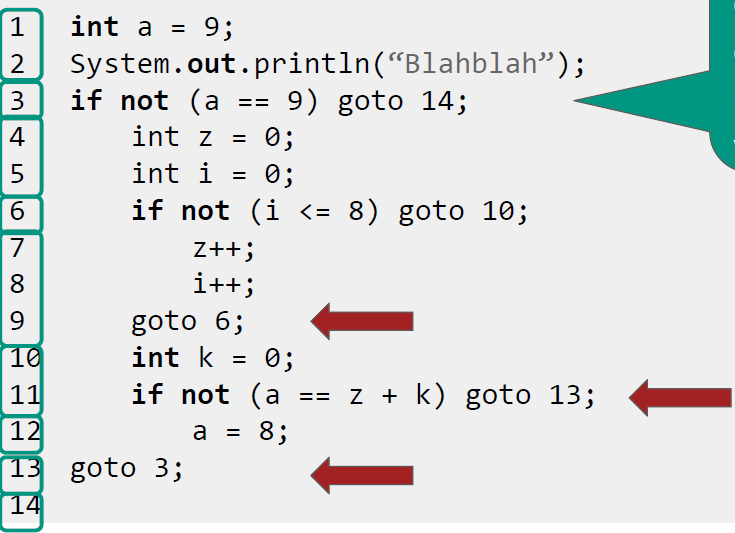
\includegraphics[scale=0.34]{./pics/tut5/second-blocks.png}
	\end{frame}

	\begin{frame}
		\frametitle{KFO: Zwischensprache nach Kontrollflussgraph}
		\begin{itemize}
			\item Grundblöcke benennen
			\item Grundblöcke und Verzweigungen hinzeichnen
			\item Start- und Endzustand hinzufügen
		\end{itemize}
	\end{frame}

	\begin{frame}
		\frametitle{KFO: Zwischensprache nach Kontrollflussgraph}
		\centering 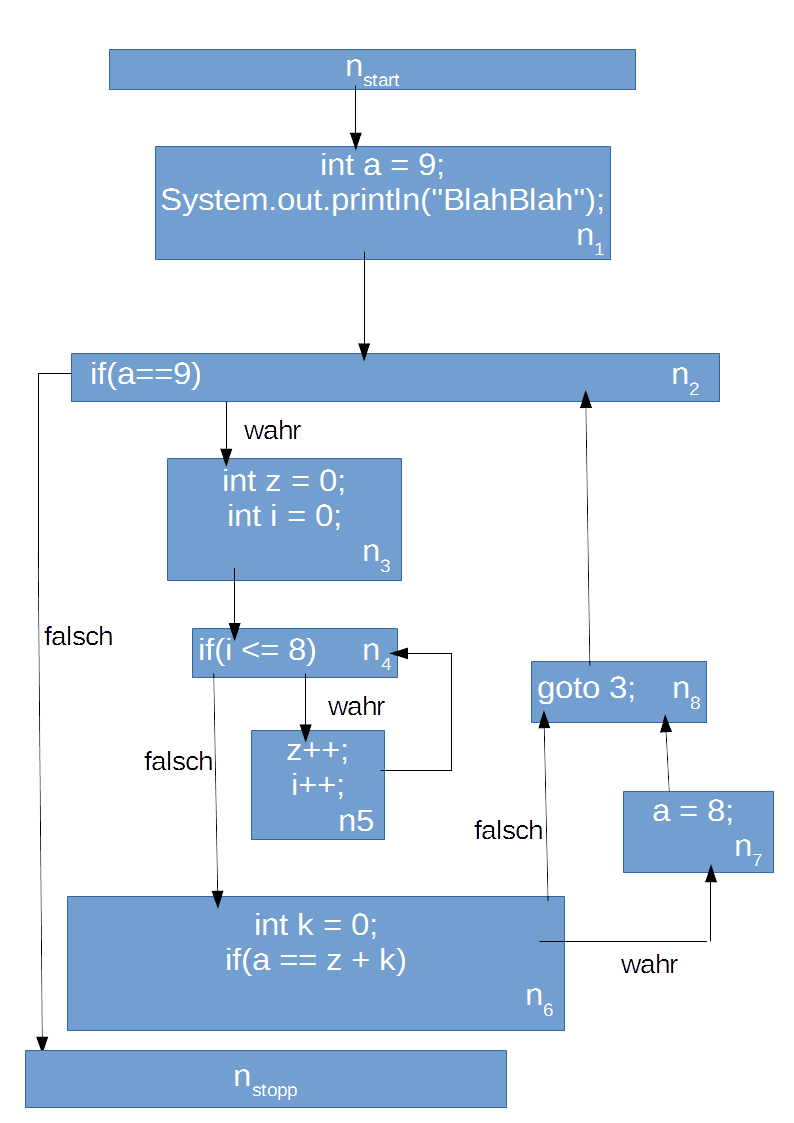
\includegraphics[scale=0.25]{./pics/tut5/test.png}
	\end{frame}

	\begin{frame}
		\frametitle{KFO: Zwischensprache nach Kontrollflussgraph}
		\begin{itemize}
			\item goto-Knoten kann man auch weglassen
		\end{itemize}
		\centering 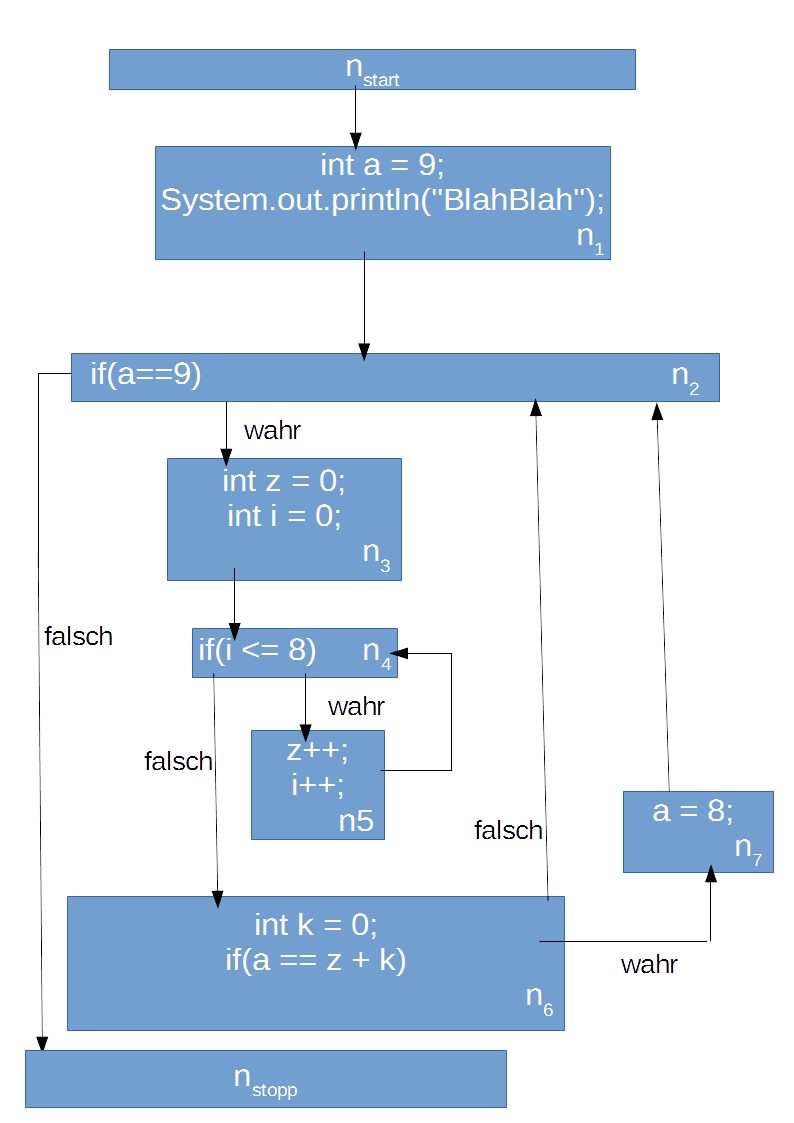
\includegraphics[scale=0.2]{./pics/tut5/test-without-goto.png}
		\pause
	\end{frame}

	\begin{frame}
		\frametitle{KFO: Anweisungsüberdeckung}
		\begin{itemize}
			\item Pfade finden, sodass jeder Grundblock traversiert wird \pause
			\linebreak $\implies$ Entdeckung nicht erreichbarer Code-Abschnitte \pause
			\item aber: kein ausreichendes Testkriterium
		\end{itemize}
	\end{frame}

	\begin{frame}
		\frametitle{KFO: Anweisungsüberdeckung}
		\centering 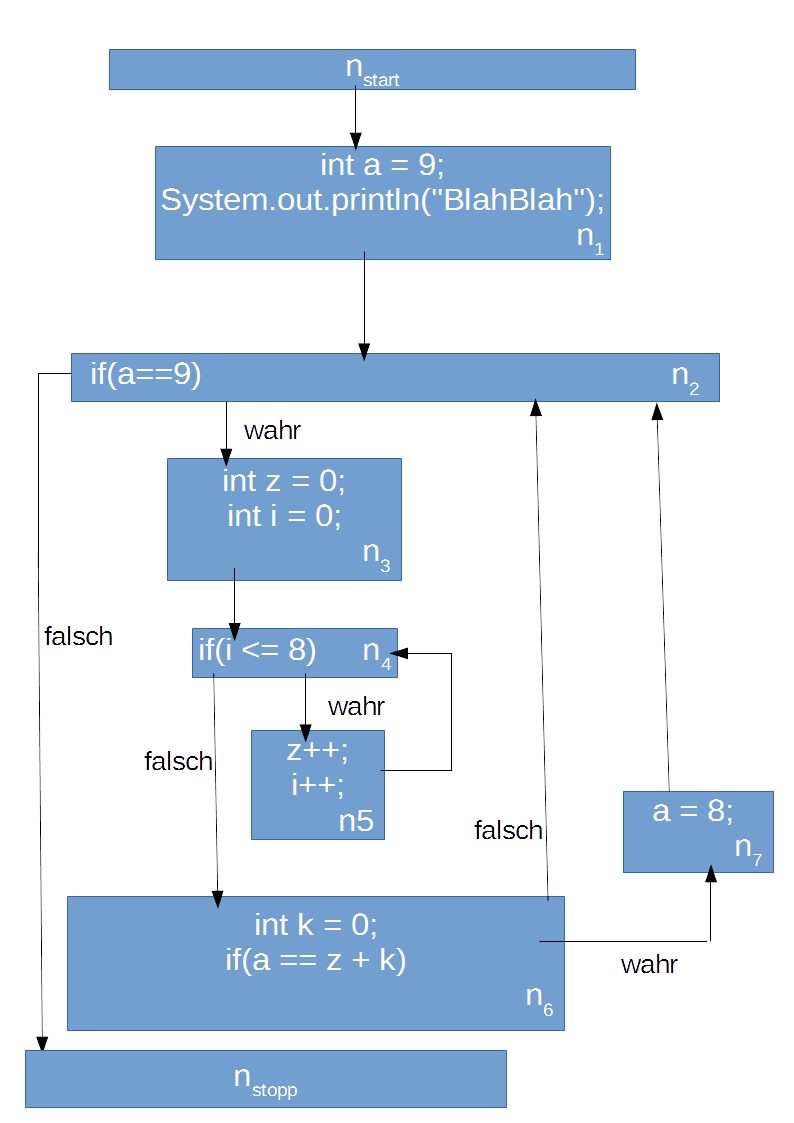
\includegraphics[scale=0.2]{./pics/tut5/test-without-goto.png}
		\begin{itemize}
			\item Pfad für Anweisungsüberdeckung? \pause ($n_{start}, n_1, n_2, n_3, n_4, n_5, n4, n_6, n_7, n_2, n_{stopp}$) 
		\end{itemize}
	\end{frame}

	\begin{frame}
		\frametitle{KFO: Zweigüberdeckung}
		\begin{itemize}
			\item Pfade finden, sodass jeder Zweig (=Kante) traversiert wird \pause
			\linebreak $\implies$ Entdeckung nicht erreichbarer Kanten \pause
			\item aber: Schleifen werden nicht ausreichend getestet
		\end{itemize}
	\end{frame}

	\begin{frame}
		\frametitle{KFO: Zweigüberdeckung}
		\centering 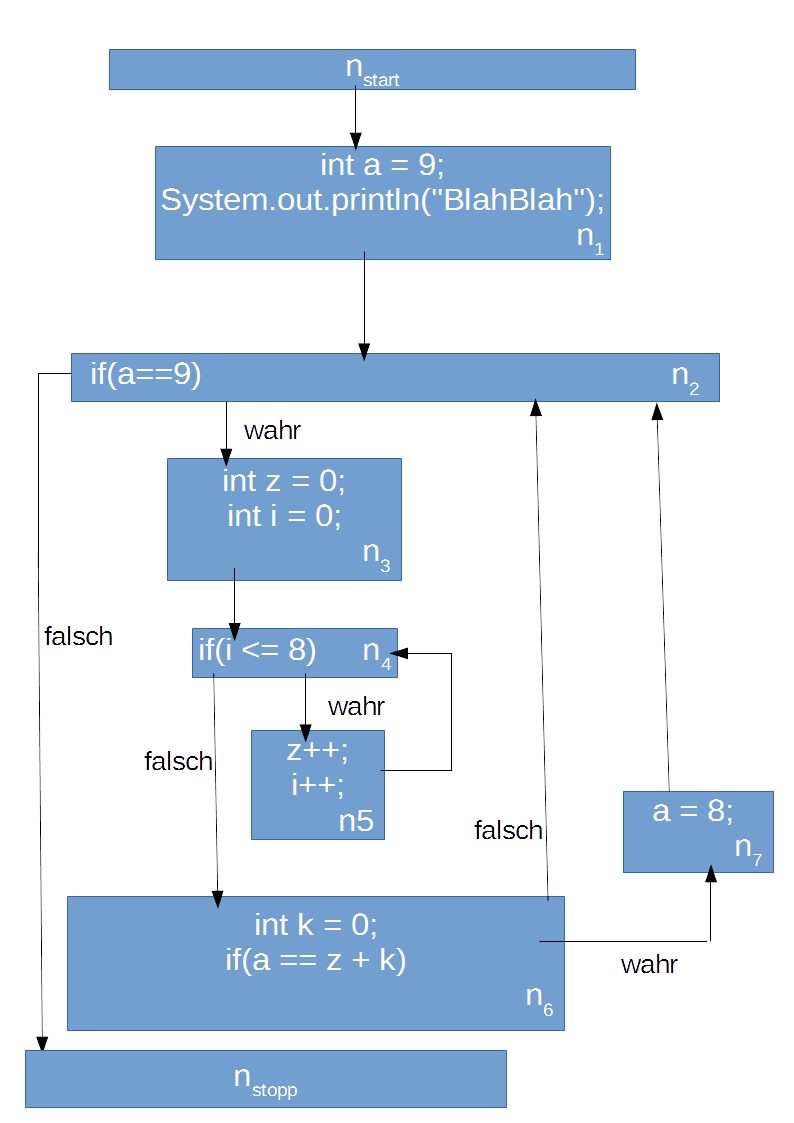
\includegraphics[scale=0.2]{./pics/tut5/test-without-goto.png}
		\begin{itemize}
			\item Pfad für Zweigüberdeckung? \pause ($n_{start}, n_1, n_2, n_3, n_4, n_5, n_4, n_6, n_2, n_3, n_4, n_5, n_4, n_6, n_7, n_2, n_{stopp}$) 
		\end{itemize}
	\end{frame}

	\begin{frame}
		\frametitle{KFO: Pfadüberdeckung}
		\begin{itemize}
			\item Finde \textbf{alle} vollständige, unterschiedlichen Pfade \pause
			\item vollständiger Pfad = Anfang bei $n_{start}$, Ende bei $n_{stopp}$ \pause
			\item nicht praktikabel, da 
			\begin{itemize}
				\item Schleifen die Anzahl der möglichen Pfade stark erhöhen \pause
				\item manche Pfade nicht ausführbar sind (sich gegenseitig ausschließende Bedingungen) \pause
			\end{itemize}
		\end{itemize}
	\end{frame}

		
	\begin{frame}
		\centering
		\begin{huge}
			Klausuraufgabe SS11
		\end{huge}
	\end{frame}


\section{Tipps}
	\subsection{Tipps}
	\begin{frame}
		\frametitle{Tipps - 6. Übungsblatt}
		\begin{exampleblock}{Aufgabe 1: Kontrollfluss-orientiertes Testen}
			\begin{itemize}
				\item Zwischensprache benutzen
				\item Definitionen der verschiedenen Abdeckungen anschauen
			\end{itemize}
		\end{exampleblock}
		\pause
		\begin{exampleblock}{Aufgabe 2: Codeinspektion} 
			\begin{itemize}
				\item an das Format halten
			\end{itemize}
		\end{exampleblock}
	\end{frame}

	\begin{frame}
		\frametitle{Tipps - 6. Übungsblatt}
		\begin{exampleblock}{Aufgabe 3: Parallelisierung von Geometrify}
			\begin{itemize}
				\item Berechnung der Samples parallelisieren
				\item Zahl der benutzten Threads abhängig machen von der Anzahl der Prozessor-Kerne
			\end{itemize}
		\end{exampleblock}
		\pause
		\begin{exampleblock}{Aufgabe 4: Alternative Parallelisierungsverfahren}
			\begin{itemize}
				\item theoretische Überlegungen, was man sonst noch so parallelisieren könnte
				\item Sinnhaftigkeit, Aufwand, etc. prüfen
			\end{itemize}
		\end{exampleblock}
	\end{frame}

	\begin{frame}
		\frametitle{Tipps - 6. Übungsblatt}
		\begin{exampleblock}{Aufgabe 5: Parallelisierungswettbewerb}
			\begin{itemize}
				\item Aufgabe 3 verbessern und Laufzeit messen
			\end{itemize}
		\end{exampleblock}
	\end{frame}

	\subsection{Abgabe}
	\begin{frame}
		\frametitle{Denkt dran!}
		\begin{alertblock}{Abgabe}
			\begin{itemize}
				\item Deadline am 19.7. um 12:00
				\item Aufgabe 1,2,4 und Beschreibung, Laufzeitprofil von Aufgabe 5 handschriftlich
			\end{itemize}
		\end{alertblock}
	\end{frame}

	\begin{frame}
		\frametitle{Bis dann! (dann  := 24.07.17)}
		\centering
		
\includegraphics[scale=1.0]{./comics/geek_and_poke_concurrency.jpg}
	\end{frame}

\end{document}